\subsection{Módulo Decoder}
	\label{sec:decoder}
	
	El módulo \textit{Decoder} (ver Figura \ref{fig:GeneralSystem}) es el encargado de demultiplexar la trama \textit{packet}[N] ya validada por el módulo \textit{Detector}. El módulo \textit{Decoder} recibe el vector de elementos booleanos \textit{packet}[N] y la señal \textit{process} que indica cuando puede iniciar el proceso de demultiplexación. La salida serán todos los vectores de estado de los elementos ferroviarios. El diagrama de bloques de la máquinas de estado finitas con camino de datos se muestra en la Figura \ref{fig:Decoder_module}.
	
	\begin{figure}[H]
		\centering
		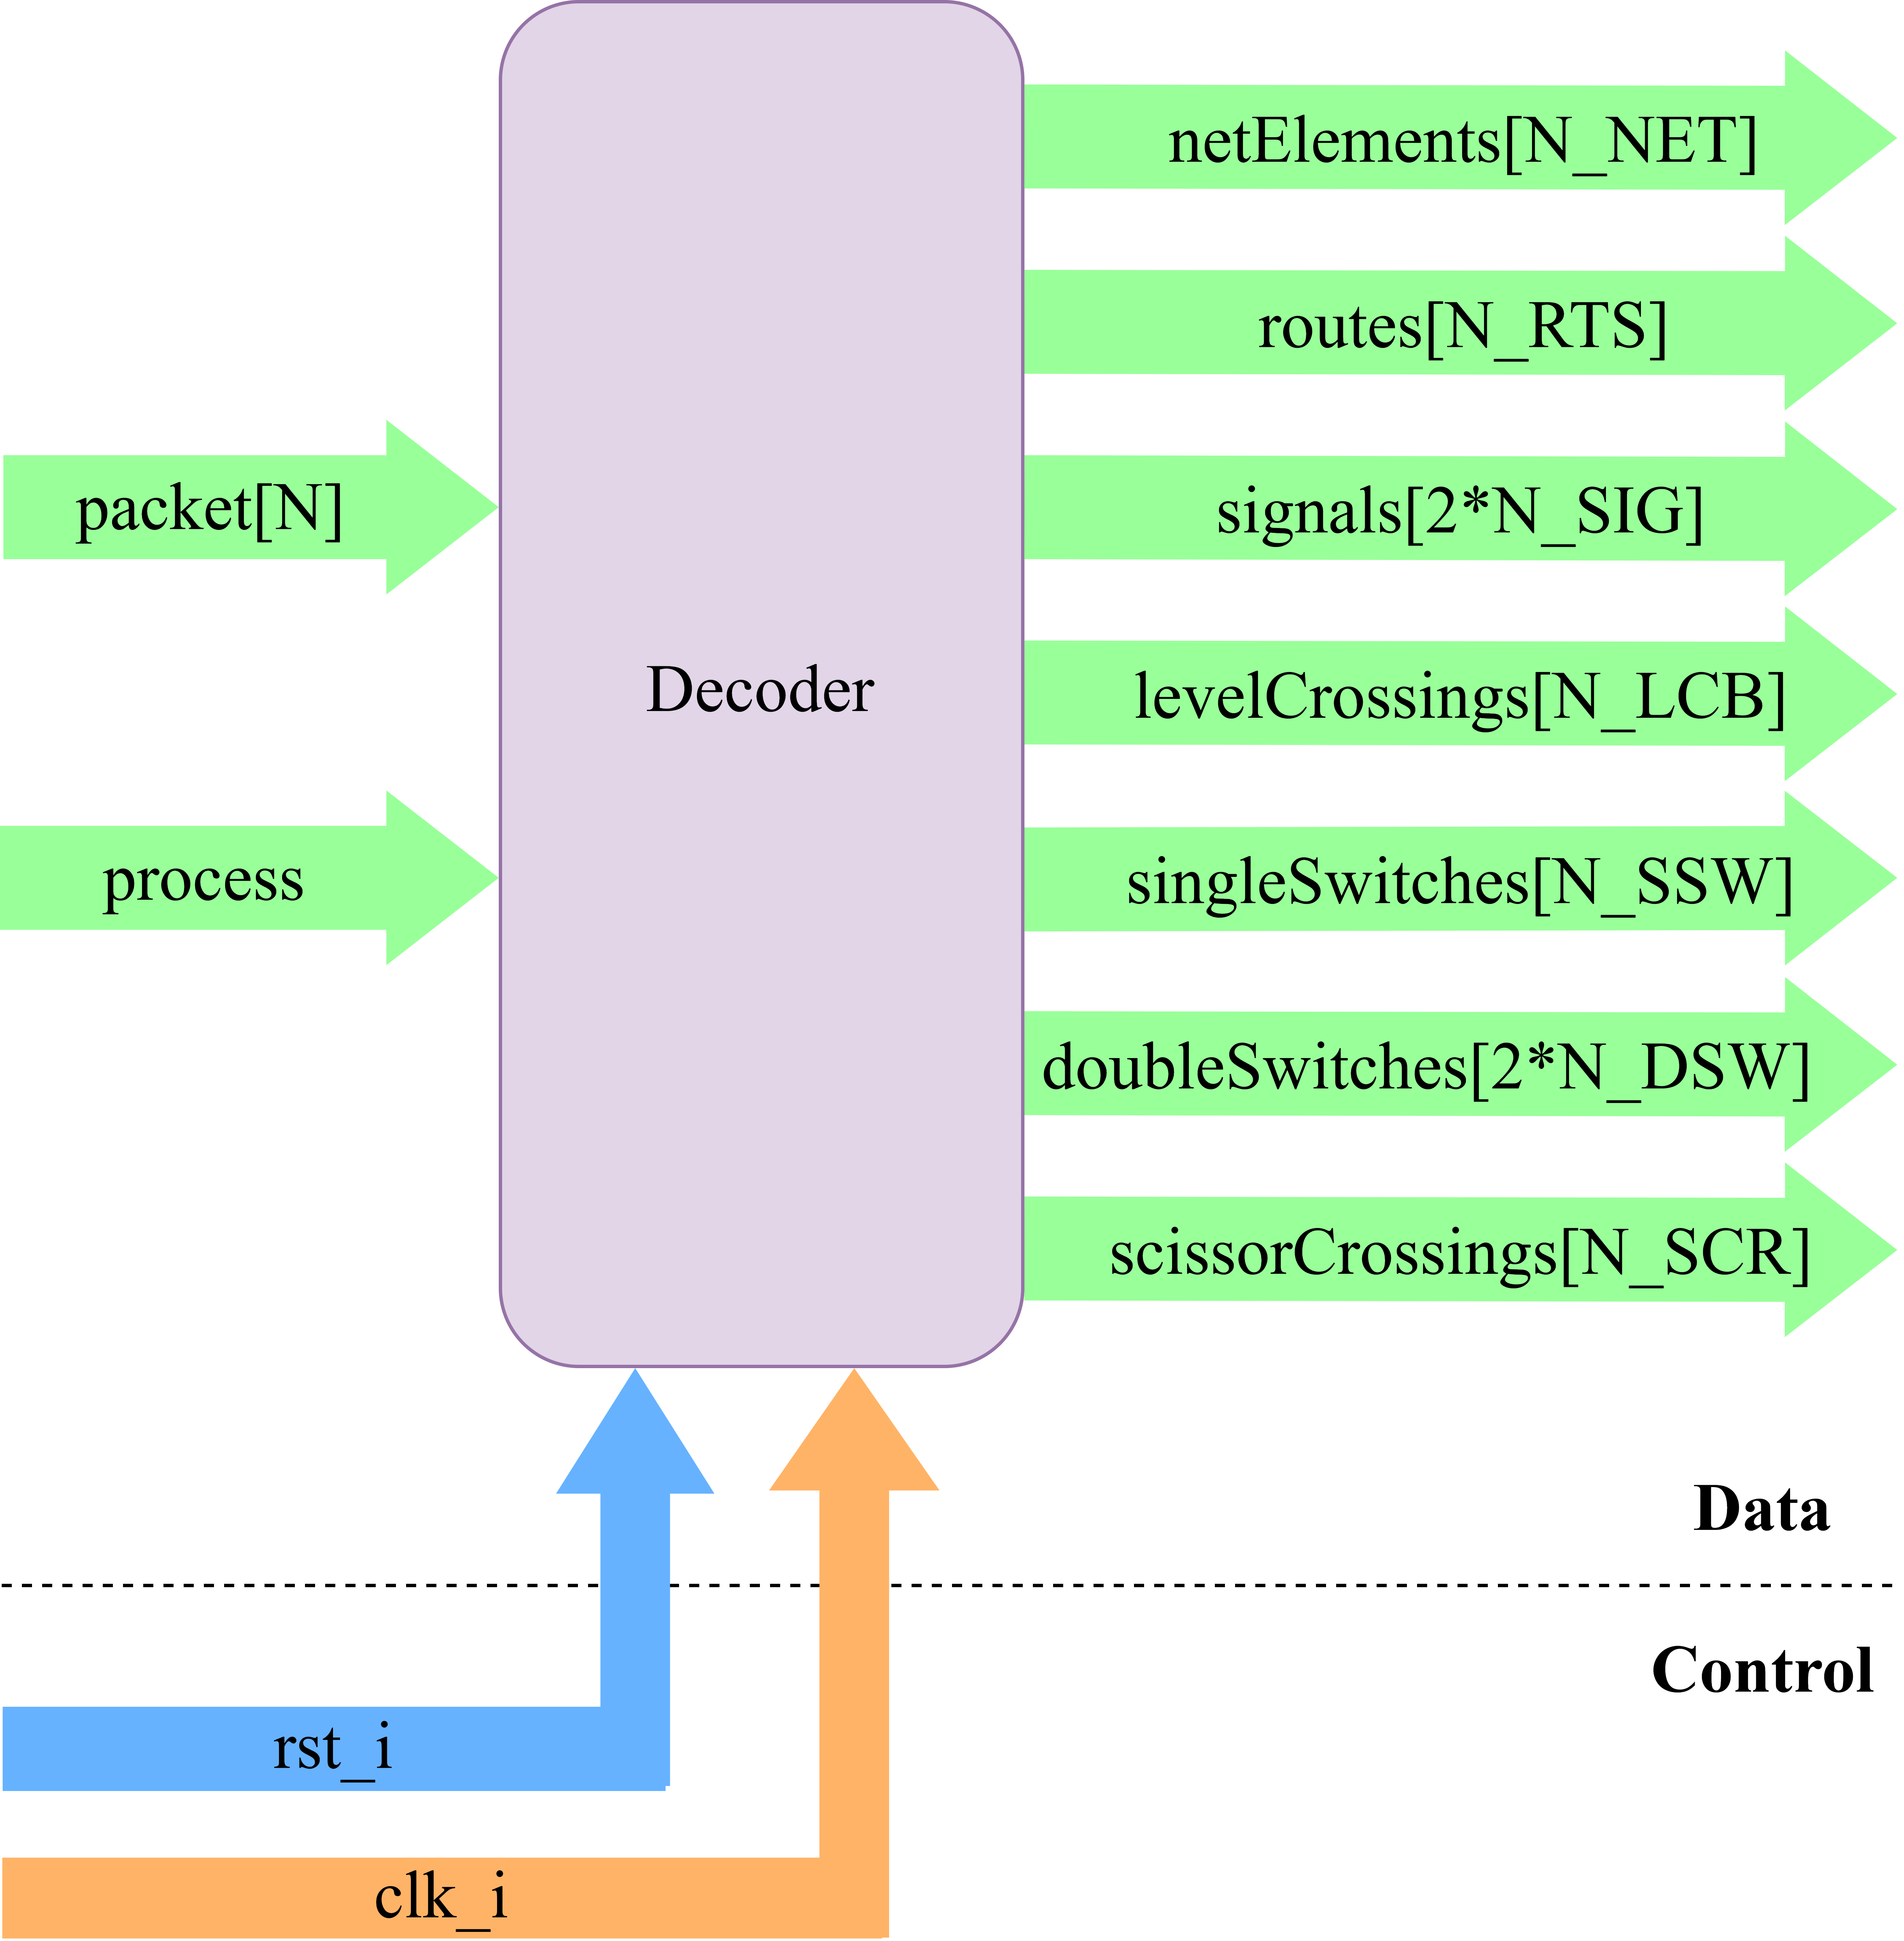
\includegraphics[width=1\textwidth]{Figuras/Decoder_module.png}
		\centering\caption{FSMD del módulo \textit{Decoder}.}
		\label{fig:Decoder_module}
	\end{figure}
	
	 La porción de \textit{packet}[N] correspondiente a cada vector será en función de la cantidad de elementos de cada tipo presentes en la locación. Esto ya fue calculado previamente por el ACG y explicado en la Sección \ref{sec:UART} al definir el formato de la trama. Si la cantidad de un cierto elemento ferroviario es mayor que uno, el ACG implementará el estado de ese elemento con un vector hexadecimal del tamaño adecuado. Si solo existe un elemento ferroviario de ese tipo, el ACG implementará un escalar hexadecimal. Si no existiese ningún elemento ferroviario en la locación, el ACG no implementará ninguna de las funcionalidades relativas a dicho elemento, optimizando el uso de recursos en la FPGA.